\section{Ergebnisse}


\begin{frame}
    \frametitle{Algorithmus}
    \begin{algorithm}[H]
        {\small
        \SetAlgoLined
        Input $\theta_{1}$,$\theta_{2}$ ,$\phi$\\
        $\overline{\theta_{1}} \leftarrow  \theta_{1}$ ,
        $\overline{\theta_{2}} \leftarrow \theta_{2}$ ,
        $\mathcal{D} \leftarrow \emptyset$\\
        \For{each iteration}{
             \For{each environment step}{
                  $a_{t}\sim \pi_{\phi}(a_{t}|s_{t})$,
                  $s_{t+1}\sim p(s_{t+1}|s_{t},a_{t})$\\
                  $D \leftarrow D \cup \{(s_{t},a_{t},r(s_{t},a_{t}),s_{t+1})\}$\\
             }
             \For{each gradient step}{
                $\theta_{i} \leftarrow \theta_{i}-\lambda_{Q}\hat{\nabla}_{\theta_{i}}J_{Q}(\theta_{i})$ for $i \in \{1,2\}$ \\
                $\phi \leftarrow \phi - \lambda_{\pi}\hat{\nabla}_{\phi}J_{\pi}(\phi)$\\
                $\alpha \leftarrow \alpha - \lambda\hat{\nabla}_{\alpha}J(\alpha)$\\
                $\overline{\theta_{i}} \leftarrow \tau\theta_{i} + (1-\tau)\overline{\theta_{i}}$ for $i \in \{1,2\}$ \\
            }
        }
        }
         \caption{Soft Actor-Critic}
        \end{algorithm}
     
\end{frame}

\begin{frame}{Ziel der Experimente}
        \begin{itemize}
            \item Stabilität und Sample Komplexität im Vergleich zu anderen Algorithmen
            \begin{itemize}
                \item Kontinuierliche Aufgaben
                \item Verschiedene Schwierigkeitgrade
            \end{itemize}  
            \item OpenAI gym und rllab
        \end{itemize}
\end{frame}

\begin{frame}{Vergleich zu anderen Algorithmen}
    \begin{itemize}
        \item SAC
        \begin{itemize}
            \item Durchschnittswert (mean action)
            \item Feste und variable Temperatur (Anpassung im neuen Paper)
        \end{itemize} 
        \item PPO, DDPG
        \begin{itemize}
            \item Kein Exploration noise
        \end{itemize}
        \item TD3
        \item SQL mit zwei Q Funktionen
        \begin{itemize}
            \item Evaluation mit Exploration noise        
        \end{itemize}
    \end{itemize}
\end{frame}

\begin{frame}{Vergleich zu anderen Algorithmen}
    \begin{itemize}     
        \item 5 Instanzen mit einer Evaluation alle 1000 Schritte
        \item Schattierter Verlauf zeigt min und max der fünf Durchläufe
    \end{itemize}
    
\end{frame}

\begin{frame}
    \frametitle{Ergebnisse}
    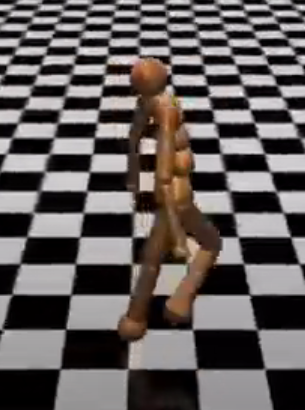
\includegraphics[width=.3\textwidth, height=0.4\textheight]{figures/rllab/Humanoid-v1.PNG}\hfill
    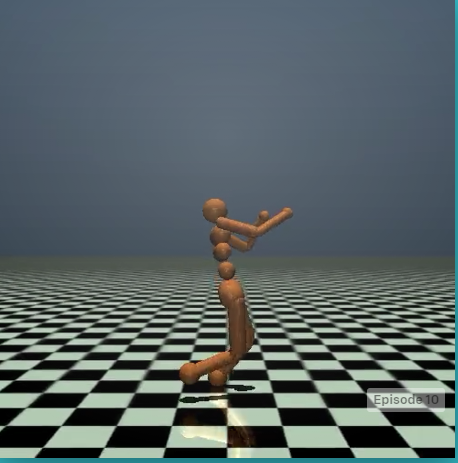
\includegraphics[width=.3\textwidth, height=0.4\textheight]{figures/rllab/Humanoid-v2.PNG}\hfill
    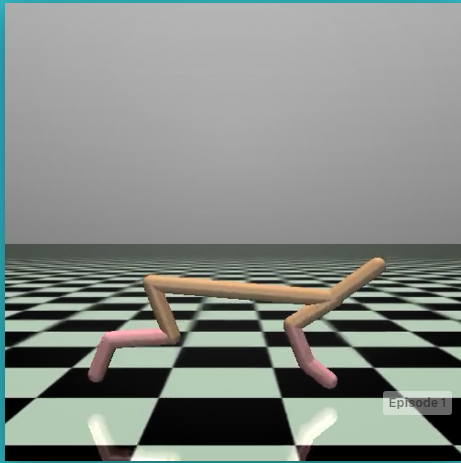
\includegraphics[width=.3\textwidth, height=0.4\textheight]{figures/rllab/halcheeathPNG.PNG}

    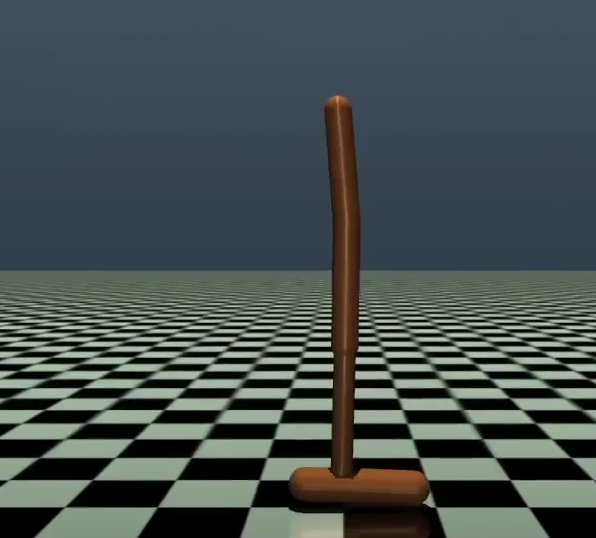
\includegraphics[width=.3\textwidth, height=0.4\textheight]{figures/rllab/Hopper.PNG}\hfill
    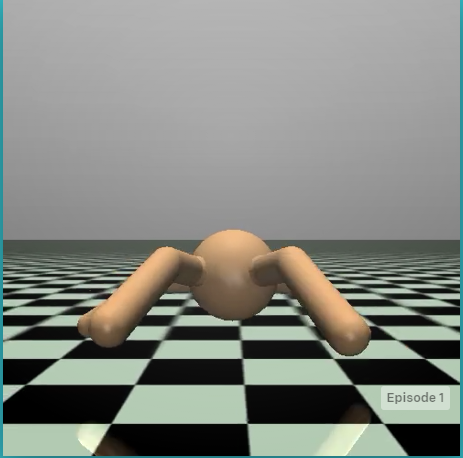
\includegraphics[width=.3\textwidth, height=0.4\textheight]{figures/rllab/antv2.PNG}\hfill
    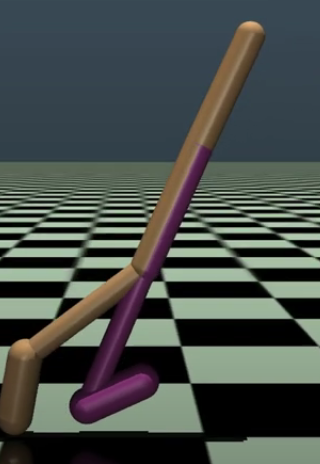
\includegraphics[width=.3\textwidth, height=0.4\textheight]{figures/rllab/walker.PNG}\hfill \\
    \cite{picturesrllab}
\end{frame}


\subsection{Vergleich mit anderen Algortihmen}
\note{
    DDPG = Deep Deterministic Policy Gradiend 
    TD3 =  Twin deep Deterministic gradiend
    PPO = Proximal Policy Optimization
}
\begin{frame}
    \frametitle{Ergebnisse}
    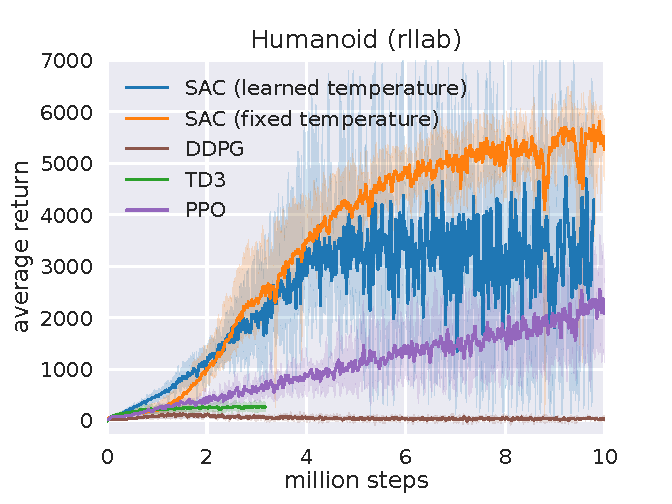
\includegraphics[width=.3\textwidth]{figures/humanoid-rllab.pdf}\hfill
    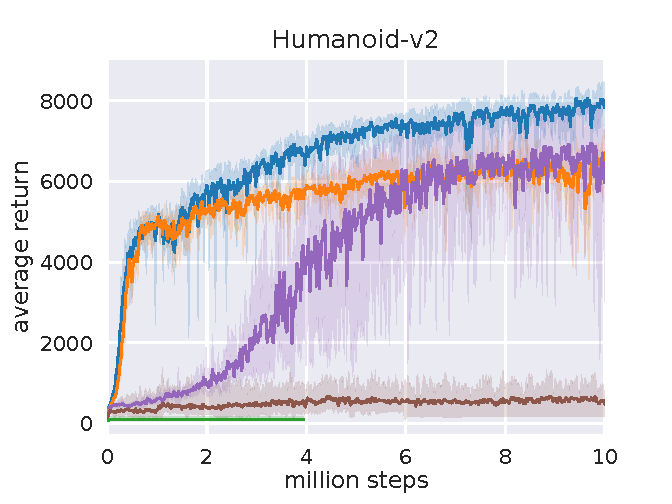
\includegraphics[width=.3\textwidth]{figures/humanoid-gym.pdf}\hfill
    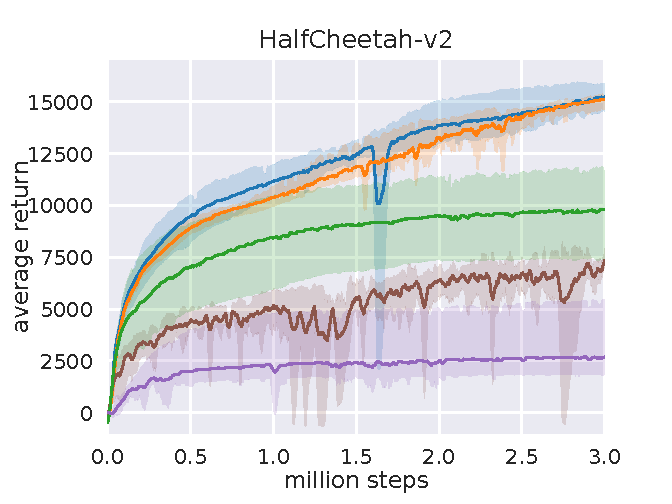
\includegraphics[width=.3\textwidth]{figures/half-cheetah.pdf}

    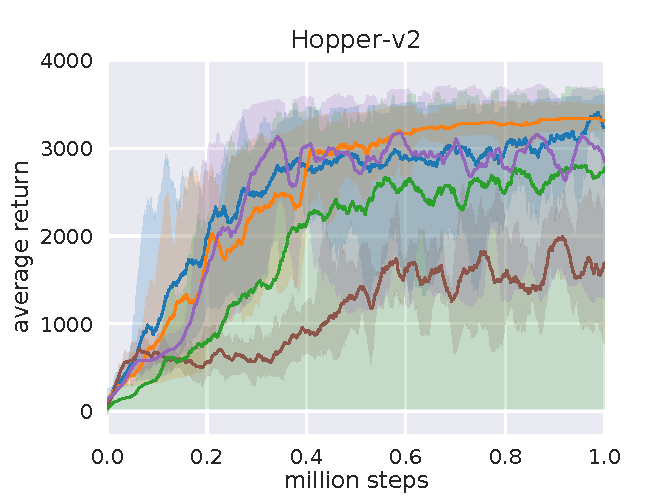
\includegraphics[width=.3\textwidth]{figures/hopper.pdf}\hfill
    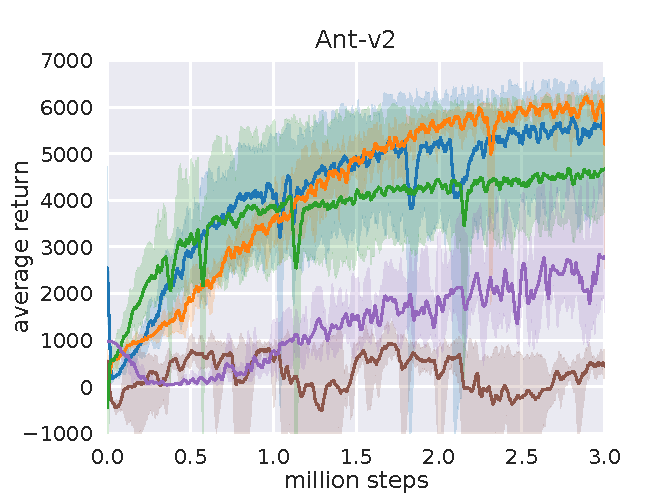
\includegraphics[width=.3\textwidth]{figures/ant.pdf}\hfill
    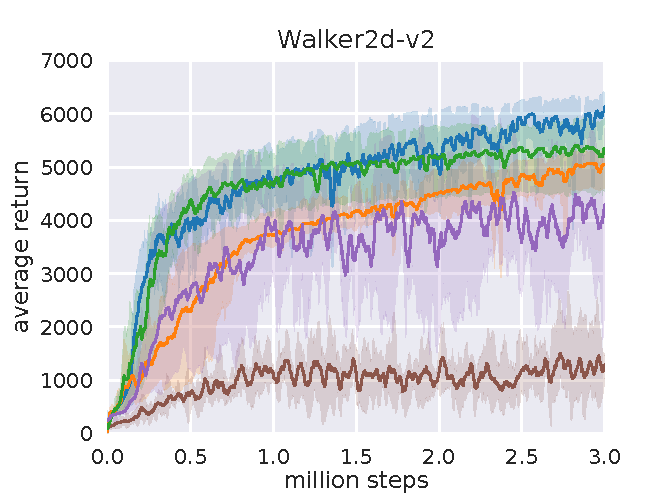
\includegraphics[width=.3\textwidth]{figures/walker.pdf}\hfill
    \cite{DBLP:journals/corr/abs-1812-05905}
\end{frame}

%\begin{frame}
%    \frametitle{Ergebnisse}
%    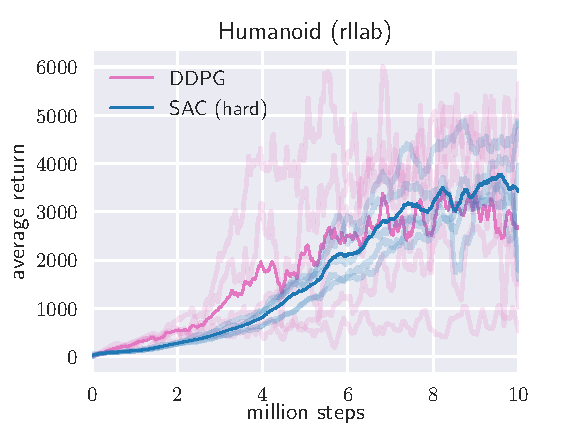
\includegraphics[width=0.8\textwidth]{figures/seeds-humanoid.pdf}
%\end{frame}


\subsection{Zusammenfassung}
\begin{frame}{Zusammenfassung}
        \begin{itemize}
            \item Soft actor critic vorgestellt
            \begin{itemize}
                \item Off policy Algorithmus
                \item Entropiemaximierung verbessert Stabilität
                \item Besser als state-of-the-art Algorithmen 
                \item Gradientenbasiertes Temperatur Tuning
            \end{itemize} 
        \end{itemize}
\end{frame}

